\documentclass[11pt]{article}

%Don't change any thing before \begin{document}
%In fact if you use sth fancy, you might need
%to add more packages, or macros.
\usepackage{amssymb,amsmath,amsthm}
\usepackage{times,psfrag,epsf,epsfig,graphics,graphicx}
\usepackage{algorithm}
\usepackage{algorithmic}

\title{CSCI 338: Assignment~3~(7 points)}
\author{River Kelly}
\date{Thursday, March 11}

\begin{document}
\maketitle

\newpage
\section*{Problem 1}
\noindent
Design context-free grammars for the following languages
\newline
\newline
\noindent
\textbf{(1.1)} $A=\{a^nb^m|n\neq 2m\}$.
\newline
\newline
$S \rightarrow aaSb \mid A \mid B \mid ab$
\newline
$A \rightarrow aA \mid a$
\newline
$B \rightarrow bB \mid b$
\newline
\newline
\noindent
\textbf{(1.2)} $B=\{a^ib^jc^k|i,j,k\geq 0$ and either $i=j$ or $j=k\}$.
\newline
\newline
$S \rightarrow AC \mid BD$
\newline
$A \rightarrow aAb \mid \epsilon$
\newline
$C \rightarrow cC \mid \epsilon$
\newline
$B \rightarrow aB \mid \epsilon$
\newline
$D \rightarrow bDc \mid \epsilon$
\newline
\newline
\noindent
\textbf{(1.3)} $C=\{a^nb^m|n=3m\}$.
\newline
\newline
$S \rightarrow aaaSb \mid \epsilon$
\newline
\newline
\noindent
\textbf{(1.4)} $D=\{a^nb^m|n\leq m+3\}$.
\newline
\newline
$S \rightarrow X \mid aX \mid aaX \mid aaaX $
\newline
$X \rightarrow  aXb \mid \epsilon $
\newline
$Y \rightarrow bY \mid b $



\newpage
\section*{Problem 2}

\noindent
Decide whether the following grammar is ambiguous.
\newline
\newline
$S\rightarrow AB \mid aaB$
\newline
$A\rightarrow a \mid Aa$
\newline
$B\rightarrow b$
\newline

\begin{proof}
By definition, a string $w$ is derived \textbf{\textit{ambiguously}} in a context-free grammar if it has two or more different leftmost derivations. A context-free grammar is \textbf{\textit{ambiguous}} if it generates some string ambiguously.
\newline
\newline
\noindent
To show that the above grammar is ambiguous, we must show that there are two or more different leftmost derivations for some string.
\begin{center}
\begin{tabular}{ c | c }
 Derivation 1 & Derivation 2 \\
 \hline 
 S & S \\
 AB & aaB \\
 AaB & aab \\
 aaB &  \\
 aab &  
\end{tabular}
\end{center}
Each derivation above, using the leftmost rule, generates its own unique and distinct parse tree, each resulting in the same output.
\newline
\newline
\noindent
$\therefore$ The given grammar must be ambiguous.
\end{proof}






\newpage
\section*{Problem 3}

\noindent
Convert the following CFG G to an equivalent PDA.

$R\rightarrow XRX|S$

$S\rightarrow aTb|bTa$

$T\rightarrow XTX|X|\epsilon$

$X\rightarrow a|b$

\begin{center}
    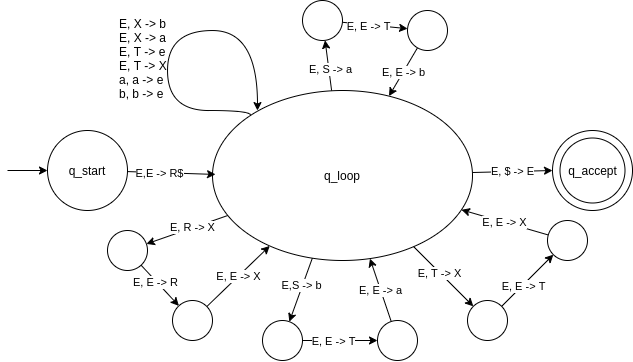
\includegraphics[scale=0.72]{HW-03-problem3.png}
\end{center}






\newpage
\section*{Problem 4}

\noindent
Let $G=(V,\Sigma,R,S)$ be the following grammar. $V=\{S,T,U\}$; $\Sigma=\{0,\#\}$; and $R$ is the set of rules:
\newline
\newline
$S\rightarrow TT|U$
\newline
$T\rightarrow 0T|T0|\#$
\newline
$U\rightarrow 0U00|\#$
\newline
\newline
\noindent
(\textbf{4.1}) Describe $L(G)$ in English.
\newline
\newline
\noindent
The language of grammar $G$, or $L(G)$, may take the form of two possibilities. The two options are described as follows:
\begin{enumerate}
  \item The first possibility is a string which contains 0's and \#'s with at least two \# symbols and any number of 0's on either side and or in between the \# symbols.
  \item The second possibility is a string beginning with $n$ zeros, the a \# symbol, and the $2n$ zeros.
\end{enumerate}
\noindent
(\textbf{4.2}) Prove that $L(G)$ is not regular.
\begin{proof}
Assume that $L(G)$ is regular. Since $L(G)$ is regular, we can apply the pumping lemma. Let $p$ be the pumping length, and let $s$ be a string such that $s \in L(G)$ where $|s| \geq p$. By definition of the pumping lemma, the following must be true:
\begin{enumerate}
  \item $xy^{i}z \in A$ for $i \geq 0$
  \item $|y| > 0$
  \item $|xy| \leq p$
\end{enumerate}
Now, we must choose $s = 0^{p}\#0^{2p} \mid s \in L(G)$.
\newline
By (2), $i = |y|$, and by (3) $|xy| \leq p$, so $y$ must consist of only zeros.
\newline
We pump up $xy^{2}z = 0^{p+i}\#0^{2p} \notin L(G)$ because the increased zeros before the \# symbol without changing those following it, so $2(p+i) \neq 2p$.
\newline
$\therefore$ A contradiction of the pumping lemma, so $L(G)$ must not be regular.
\end{proof}







\newpage
\section*{Problem 5}

\noindent
Convert the following CFG into an equivalent CFG in Chomsky Normal Form
\newline
\newline
$A \rightarrow BAB \mid B \mid \epsilon$
\newline
$B \rightarrow 00 \mid \epsilon$
\newline
\newline
\noindent
\textbf{Step 1} First, we add a new start variable $S$ and the rule $S \rightarrow A$ where
$A$ was the original start variable.
\newline
\newline
$S \rightarrow A $
\newline
$A \rightarrow BAB \mid B \mid \epsilon$
\newline
$B \rightarrow 00 \mid \epsilon$
\newline
\newline
\noindent
\textbf{Step 2} Take care and remove all $\epsilon$-rules.
\newline
\newline
\textbf{2a} Remove $B \rightarrow \epsilon$
\newline
\newline
$S \rightarrow A $
\newline
$A \rightarrow BAB \mid BA \mid AB \mid A \mid B \mid \epsilon$
\newline
$B \rightarrow 00$
\newline
\newline
\textbf{2b} Remove $A \rightarrow \epsilon$
\newline
\newline
$S \rightarrow A \mid \epsilon$
\newline
$A \rightarrow BAB \mid BA \mid AB \mid A \mid B \mid BB$
\newline
$B \rightarrow 00$
\newline
\newline
\noindent
We do not need to remove the $\epsilon$-rule $S \rightarrow \epsilon$ since $S$ is the start variable.
\newpage
\noindent
\textbf{Step 3} Handle all unit-rules. 
\newline
\newline
\textbf{3a} Remove $A \rightarrow A$
\newline
\newline
$S \rightarrow A \mid \epsilon$
\newline
$A \rightarrow BAB \mid BA \mid AB \mid B \mid BB$
\newline
$B \rightarrow 00$
\newline
\newline
\textbf{3b} Remove $A \rightarrow B$
\newline
\newline
$S \rightarrow A \mid \epsilon$
\newline
$A \rightarrow BAB \mid BA \mid AB \mid 00 \mid BB$
\newline
$B \rightarrow 00$
\newline
\newline
\textbf{3c} Remove $S \rightarrow A$
\newline
\newline
$S \rightarrow BAB \mid BA \mid AB \mid 00 \mid BB \mid \epsilon$
\newline
$A \rightarrow BAB \mid BA \mid AB \mid 00 \mid BB$
\newline
$B \rightarrow 00$
\newline
\newline
\textbf{3d} Replace ill-placed terminals by new variable $C$
\newline
\newline
$S \rightarrow BAB \mid BA \mid AB \mid CC \mid BB \mid \epsilon$
\newline
$A \rightarrow BAB \mid BA \mid AB \mid CC \mid BB$
\newline
$B \rightarrow CC$
\newline
$C \rightarrow 0$
\newline
\newline
\textbf{Step 4} Finally, convert all remaining rules into the proper form. (i.e. by replacing each rule $A \rightarrow u_{1}u_{2} \dots u_{k}$, where $k \geq 3$)
\newline
\newline
$S \rightarrow BD_{1} \mid BA \mid AB \mid CC \mid BB \mid \epsilon$
\newline
$A \rightarrow BD_{2} \mid BA \mid AB \mid CC \mid BB$
\newline
$B \rightarrow CC$
\newline
$C \rightarrow 0$
\newline
$D_{1} \rightarrow AB$
\newline
$D_{2} \rightarrow AB$
\newpage
\section*{Problem 6}

\noindent
Using pumping lemma to prove that the following languages are not
context-free.
\newline
\newline
\noindent
(\textbf{6.1}) $L=\{a^nb^jc^k|k=nj\}$.
\begin{proof}
Assume $L$ is regular, then choose $s = a^{p}b^{p}c^{p^{2}}$ where $p$ is the pumping length. By the pumping lemma, $s$ may be decomposed into $uvxyz$, such that:
\newline
\newline
(1) $uv^{i}xy^{i}z \in L$ for $i \geq 0$
\newline
(2) $|vy| > 0$
\newline
(3) $|vxy| \leq p$
\newline
\newline
There are three possible cases, let's examine each:
\begin{enumerate}
  \item $vxy$ is made up of $b$'s and $c$'s.
  \item $vxy$ does not have an $c$'s.
  \item $vxy$ contains only $c$'s.
\end{enumerate}
In case 1, pumping $uv^{2}xy^{2}z$ take the form $a^{p}b^{p+i}c^{p^{2}+j}$. Then, $p(p+i) = p^{2} + ip > p^{2} +j$ since $i > 0$, and by (3) $j > p$. Therefore $uv^{2}xy^{2}z \notin L$.
\newline
\newline
In case 2, pumping $uv^{2}xy^{2}z$ violates (2) because there would be more $a$'s or $b$'s without changing the number of $c$'s.
\newline
\newline
Lastly, in case 3, when pumping $uv^{2}xy^{2}z$ also violates (2) because there is more $c$'s without changing the number of $a$'s or $b$'s.
\newline
\newline
$\therefore$ A contradiction in all cases, so $L$ must not be regular.
\end{proof}
\newpage
\noindent
(\textbf{6.2}) $L=\{a^nb^j|n\geq (j-1)^3\}$.
\begin{proof}
Assume $L$ is regular, then choose $s = a^{(p-1)^{3}}b^{p}$ where $p$ is the pumping length. By the pumping lemma, $s$ may be decomposed into $uvxyz$, such that:
\newline
\newline
(1) $uv^{i}xy^{i}z \in L$ for $i \geq 0$
\newline
(2) $|vy| > 0$
\newline
(3) $|vxy| \leq p$
\newline
\newline
There are three possible cases, let's examine each:
\begin{enumerate}
  \item $vxy$ is made up of only $a$'s.
  \item $vxy$ contains both $a$'s and $b$'s.
  \item $vxy$ contains only $b$'s.
\end{enumerate}
In case 1, by pumping down such that, $uv^{0}xy^{0}z = uxz$. By rule (2) $i = |vy| > 0$, so $uxz$ has the form $a^{(p-1)^{3}-i}b^{p}$. But, $(p-1)^{3}-i < (p-1)^{3}$. Therefore $uxz \notin L$.
\newline
\newline
In case 2, pumping up $uv^{2}xy^{2}z$ takes the form $a^{(p-1)^{3}+i}b^{p+j}$, and we know that $j \neq 0$ so $(p-1+j)^{3} \geq (p)^{3}$. Then, $(p-1)^{3} + i < (p-1)^{3} + 3p^{2} - 3p +1 = p^{3}$ for $p > 1$. Therefore $uxz \notin L$.
\newline
\newline
In case 3, pumping up $uv^{2}xy^{2}z$ takes the form $a^{(p-1)^{3}}b^{p+i}$. Thus, increasing the number of $b$'s without altering the number of $a$'s. By (2), $i = |vy| >0$, then $(p-1)^{3} < (p+i-1)^{3}$. Therefore $uxz \notin L$.
\newline
\newline
$\therefore$ A contradiction in all cases, so $L$ must not be regular.
\end{proof}
\end{document}

